\pagebreak
\section{Daten bekommen}
\label{getData}

Auf der Website werden wiederholt Daten vom Server geholt. Dies erfolgt mittels \textit{fetch}.
Mit dem Fetch Befehl und dem richtigen API-Link werden die gebrauchten Daten vom Server geholt. 


Im Projekt wird ein Custom Fetch verwendet, welcher zusätzlich zu den Daten auch einen 
Error liefert falls der Fetch fehlschlägt, als so wohl auch eine boolean Variable, welche true ist und 
erst false wird, sobald alle Daten vom Server empfangen wurden. Diese Variable namens 
\textit{isPending} ist in dem Sinne von nützen, dass der Nutzer informiert wird, dass die Daten noch
laden müssen.
\begin{code}[htp]
\begin{lstlisting}
import { useState, useEffect } from 'react';
import Error from '../staticViews/Error'

const useFetch = url => {
  const [data, setData] = useState(null);
  const [isPending, setIsPending] = useState(true);
  const [error, setError] = useState(null);

  useEffect(() => {
    const abortCont = new AbortController();

    setTimeout(() => {
      fetch(url, {
        method: 'GET',
        signal: abortCont.signal })
        .then(res => {
          if (!res.ok) {
            throw Error('Daten konnten nicht empfangen werden');
          }
          return res.json();
        })
        .then(data => {
          setIsPending(false);
          setData(data);
          setError(null);
        })
        .catch(err => {
          if (err.name === 'AbortError') {
            console.log('fetch abgebrochen')
          } else {
            setIsPending(false);
            setError(<Error></Error>);
          }
        });
    });

    return () => abortCont.abort();
  }, [url]);

  return { data, isPending, error };
};

export default useFetch;

\end{lstlisting}
\caption{React Component - useFetch zum Empfangen von Daten}
\end{code}

Wie im Code sichtbar, werden die drei Variablen mit einem \textit{setState} und dem Wert null
deklariert. Außer \textit{isPending} welche wie oben schon genannt standardmäßig auf true ist. Diese
drei Werte werden am Ende als return Wert zurückgegeben um sie außerhalb des useFetch benutzen 
zu können.


Falls ein Fehler auftritt, wird der State der Error Variable auf eine Error Komponente gesetzt. Dies
sorgt für eine Einheitliche Fehlermeldung, falls es ein Problem beim Bekommen der Daten auftritt.

Diese Fehlermeldung sieht wie folgt aus:
\begin{figure}[H]
    \begin{center}
      \frame{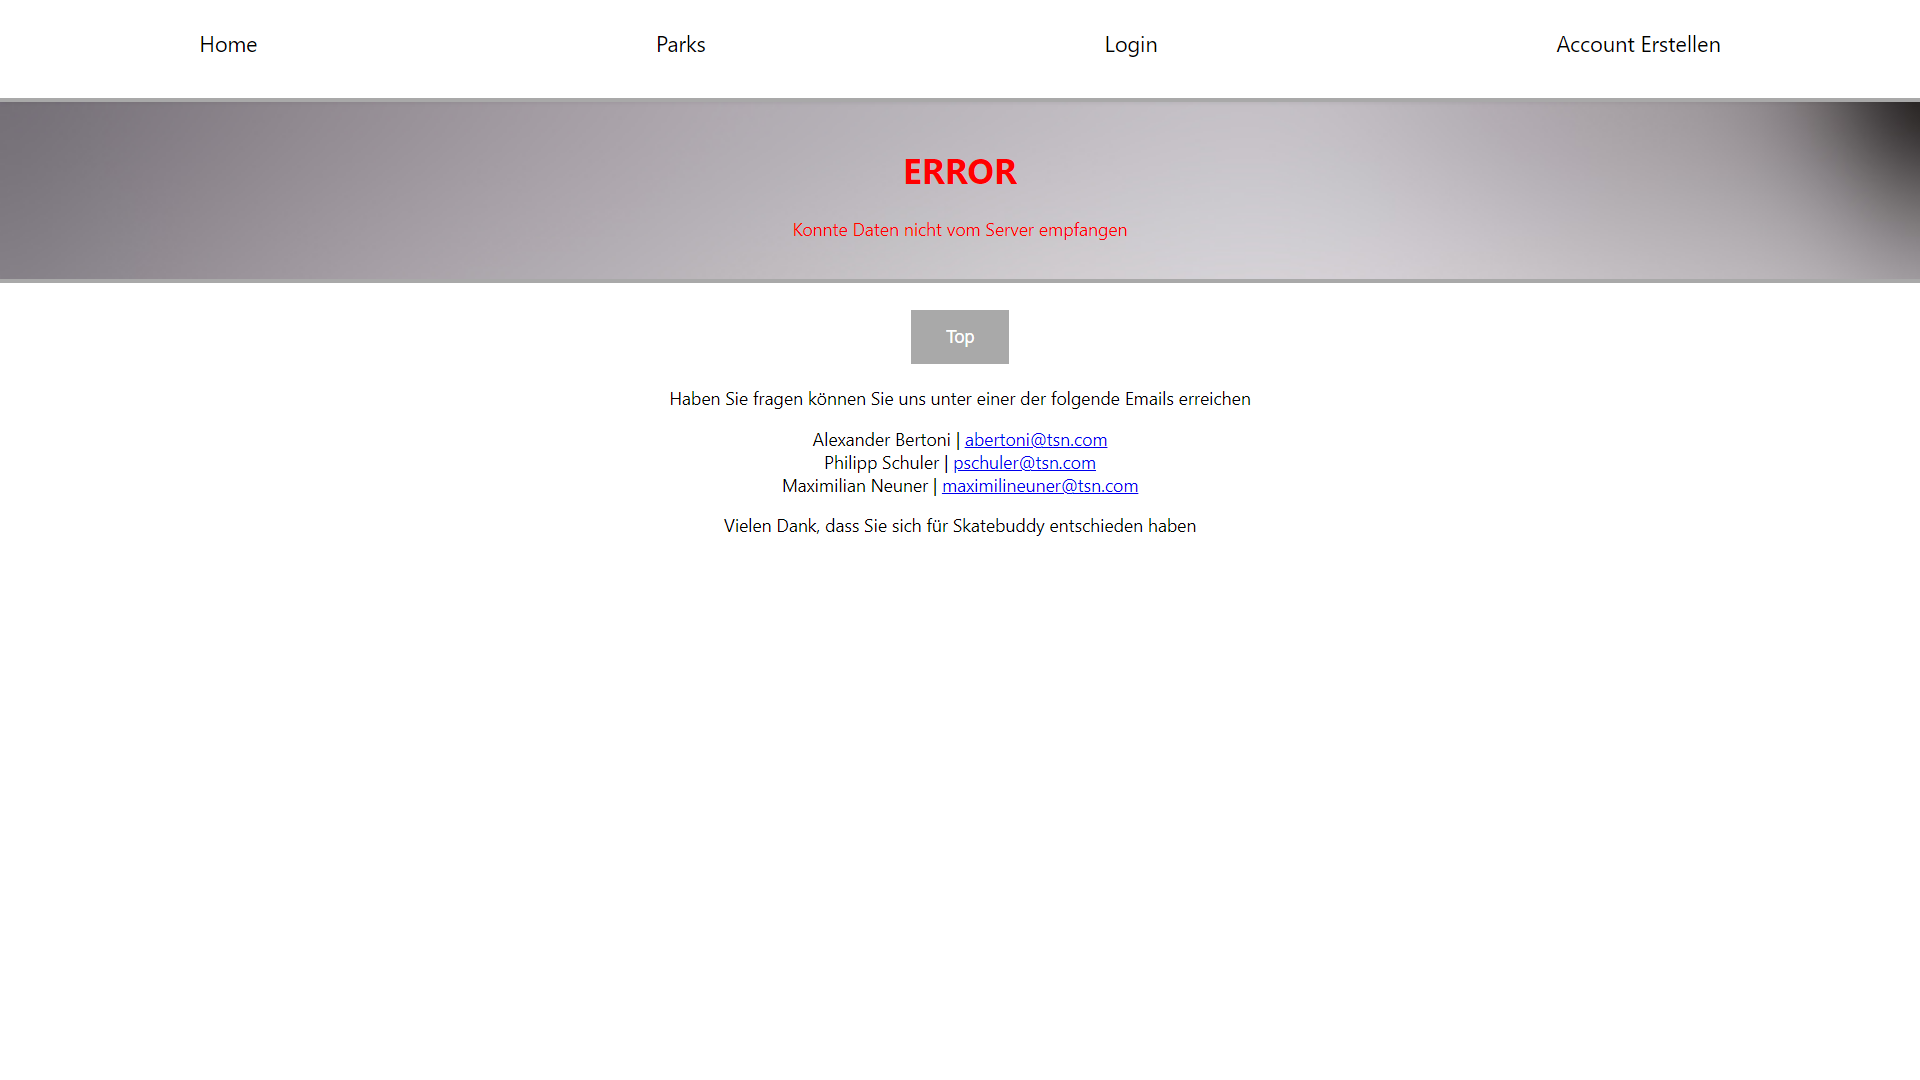
\includegraphics[width=1\textwidth]{Website/ErrorMessage.png}}
      \caption{Fehlermeldung wenn das Daten holen vom Server fehlschlägt}
    \end{center}
  \end{figure}
  